\section{Notice d'utilisation du programme}
\subsection{Compilation}

Ayant dans ma folie fait mon code que dans un seul fichier, la compilation est assez simple. Un simple gcc permet de compiler le fichier. Voici ma commande de compilation :
 \smallbreak

\textit{reset ; gcc -g -W -Wall metro.c && ./a.out}

\subsection{Execution}

A l'execution le programme fourni une liste de station et leurs ID. Puis le programme demande à l'utilisateur d'entré l'ID d'une station puis une autre.
Après peu de temps, le programme fourni un trajet (logiquement le plus cour) a faire pour arriver à destination. Elle est à lire de bas en haut.

\begin{figure}[h]
\centerline{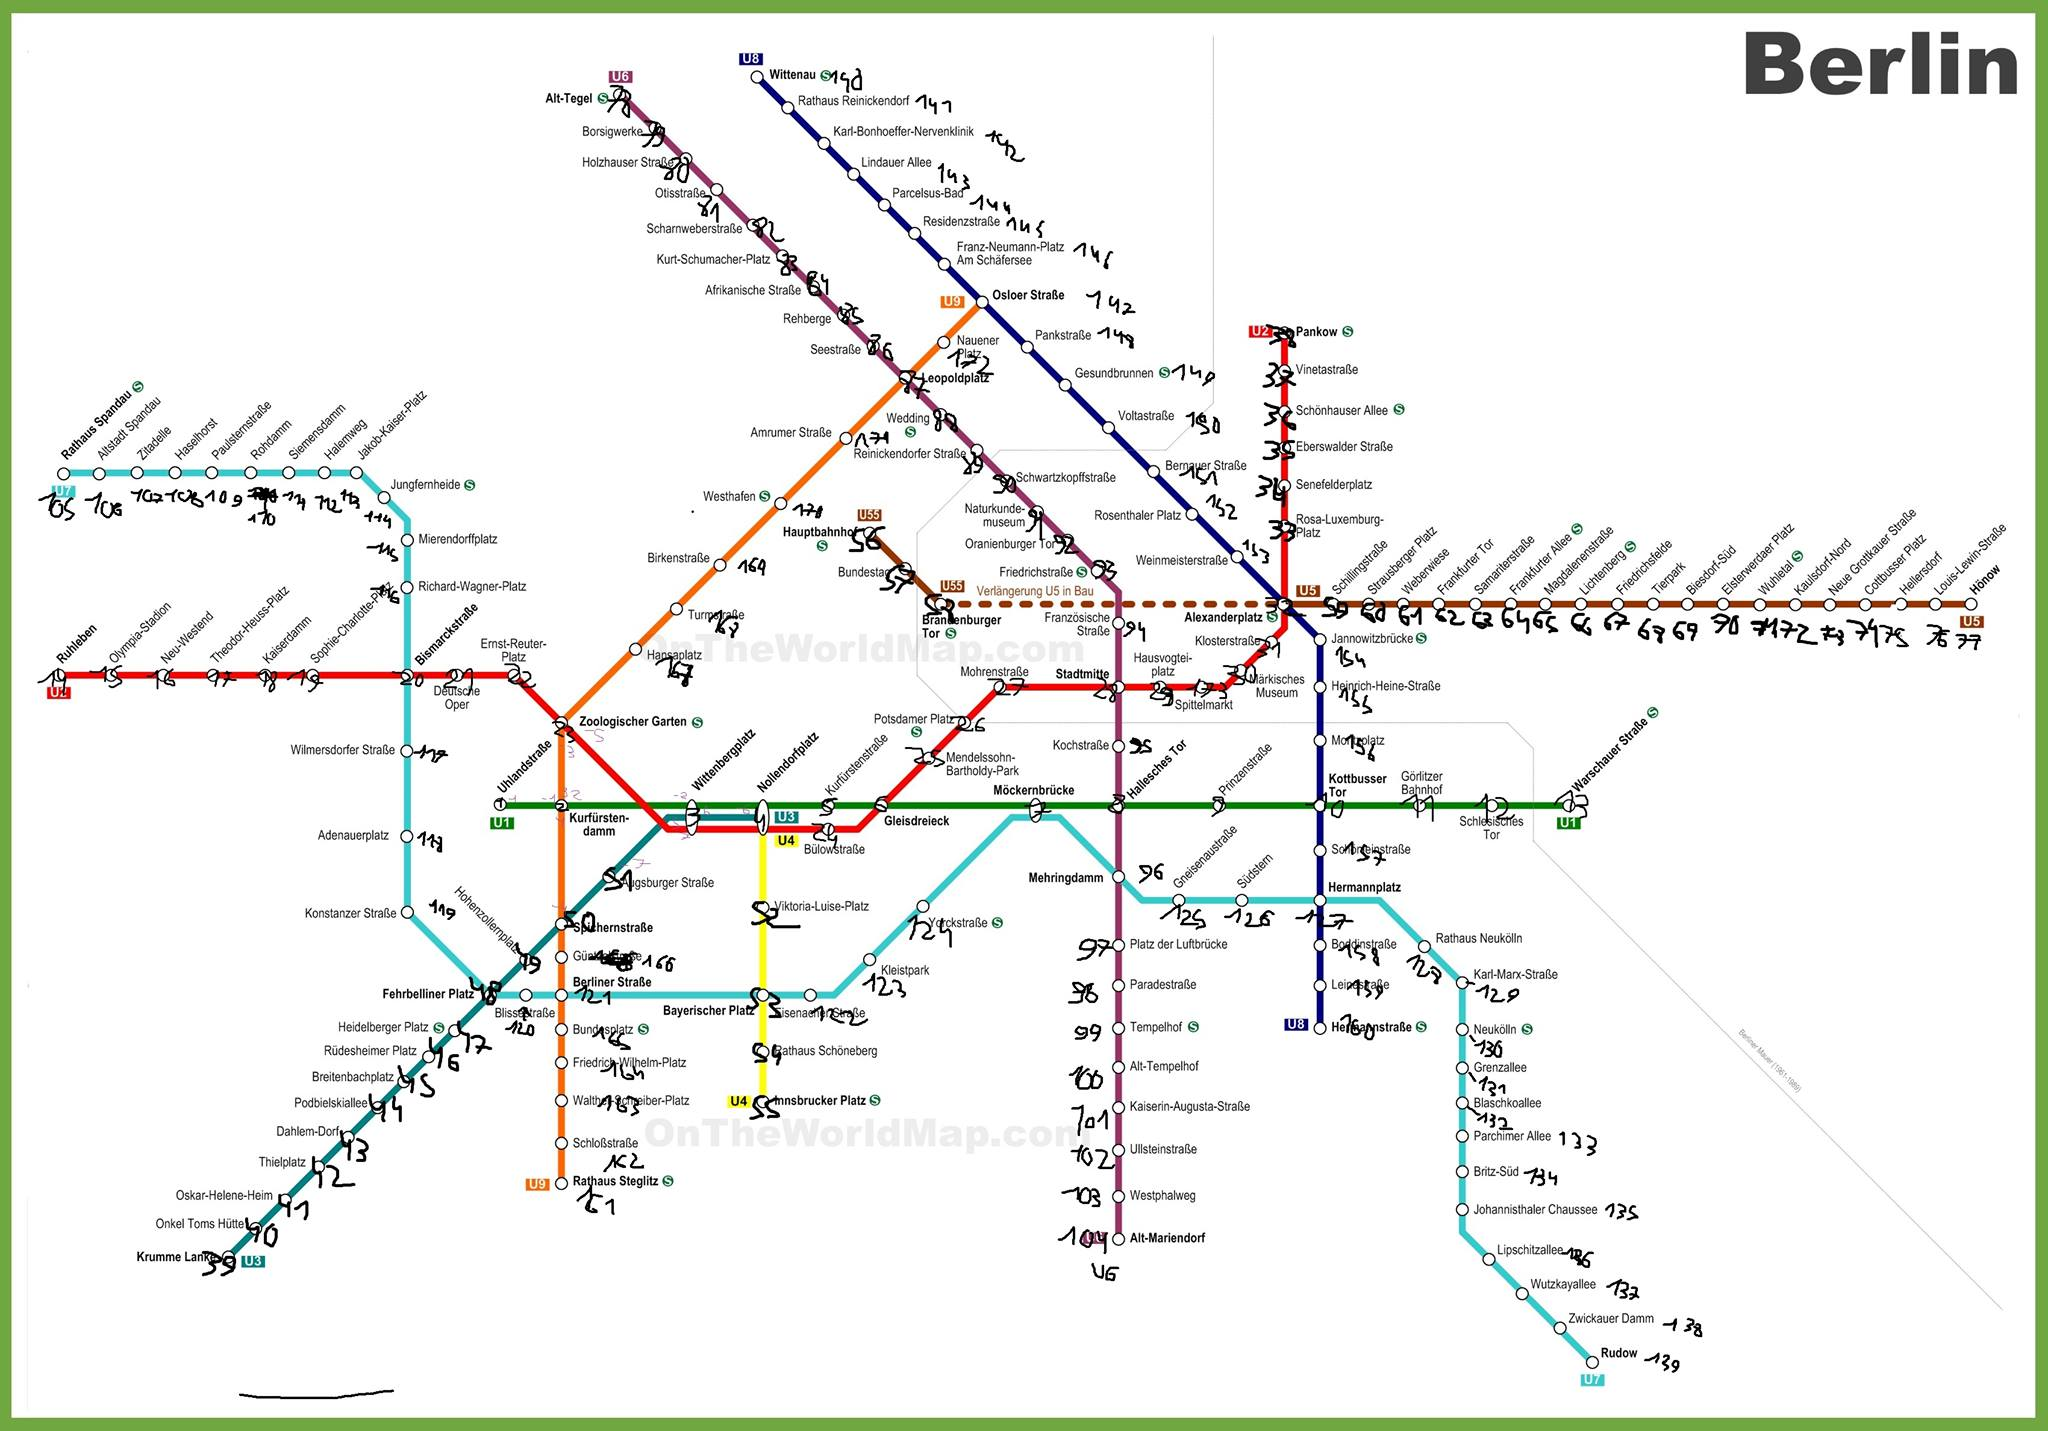
\includegraphics[width=1\textwidth]{images/metroID.jpg}}
\caption{\label{legende} Metro de berlin avec les ID.
}
\end{figure}
